\documentclass[journal,12pt,onecolumn]{IEEEtran}
\usepackage{amsmath}
\usepackage{amssymb}
\usepackage{enumerate}
\usepackage[utf8]{inputenc}
\usepackage{multicol}
\usepackage{gensymb}
\usepackage{nopageno}
\usepackage{mathtools}
\usepackage{siunitx}
\usepackage{graphicx}
\graphicspath{ {/home/diparna/Desktop/Adaptive Signal Processing} }
\newcommand\myeq{\mathrel{\stackrel{\makebox[0pt]{\mbox{\normalfont\tiny def}}}{=}}}

\begin{document}

\centering \textbf{EE608  Adaptive Signal Processing}\\

\medskip
{Problem Set 1 — Some Basic Problems in Estimation and Matrix Computation}\\
\medskip

\begin{enumerate}
\setlength{\itemsep}{2em}

\item Consider the following M-th order FIR adaptive structure for noise cancellation shown in class\\
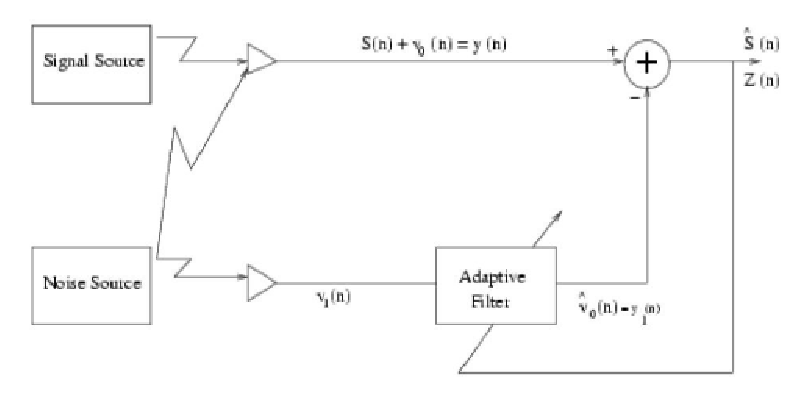
\includegraphics{figure1.eps}

Assume that $v_i(n)$ and s(n) are statistically independent.Let $e(n)=s(n)+v_0(n)-\hat{v}_0(n)$.Now suppose the adaptation rule is chosen such that $E[e^2(n)]$ is minimized.Then show that $E[e^2(n)]=E[(s(n)-\hat{s}(n))^2]$.Thus minimizing $E[e^2(n)]$ will indeed yield $\hat{s}(n)$ as the minimum mean sqaure estimate of s(n).

\item Let $\{\large{y}_k\}_{k=1}^N$ be N measurements of unknown constant c. The problem is to derive the expression for the $l_2$,$l_1$, and $l_\infty$ estimate of the constant c using the measurements $\{\large{y}_k\}_{k=1}^N$\\
We model the measurements as sample values of a discrete time random variable Y having the density function\\
                            $$f_Y(y)=\quad\sum_{k=1}^{N}{\alpha_k}{\delta(y-y_k)}$$
                             
where $\alpha_k$ are such that $\quad\sum_{k=1}^{N}{\alpha_k}=1.$\\
Show that
\begin{enumerate}[(a)]
\item The $l_2$ estimate of c is given by
$$\hat{c}=\quad\sum_{k=1}^{N}{\alpha_k}{y_k}$$
\item The $l_1$ estimate of c is given by $\hat{c}={y_p}$, for $1\leq{p}\leq{N}$ such that
$$\quad\sum_{y_k<{\hat{c}}}\alpha_{k}=\quad\sum_{y_k>{\hat{c}}}\alpha_{k}$$

\item The $l_\infty$ estimate is given by
$$\hat{c}=\frac{min\{{y_k}\}+max\{y_k\}}{2}$$
\end{enumerate}
\item Consider the problem of estimating the mean and variance of a Gaussian distributed random variable.\\

Let
$${X_k}, {k=1},... N$$\\
be N independent samples of a stationary Gaussian distribution.Thus\\
$$f_{{X_k}|{M},{V^{{(x_k}|m,{\sigma^2})}}}=\frac{1}{2\pi\sigma^2}e^{-(x_k-m)^2/(2\sigma^2)}$$
and letting $Z=\{{X_1},...,{X_N}\},z=\{x_1,...,x_n\}$
$$f_{{Z|M},{V^{{(z|m,\sigma^2})}}}=\prod_{k=1}^{N}f_{{X_k}|{M},{V^{{(x_1}|m,{\sigma^2})}}}=\frac{1}{(2\pi\sigma^2)^{N/2}}exp[-\quad\sum_{k=1}^{N}{({x_k}-m)^2}/{2\sigma^2}]$$
\begin{enumerate}[(a)]
\item Assume $\sigma^2$ is known. Show that the MLE of m is given by
$$\hat{m}_{MLE}=\frac{1}{N}\quad\sum_{k=1}^{N}x_{k}$$\\
and that is an unbiased estimate.
\item Assume m is known. Show that MLE of  $\hat{\sigma^2}$ is given by
$$(\hat{\sigma^2})_{MLE}=\frac{1}{N}\quad\sum_{k=1}^{N}({x_k}-m)^2$$\\
and that is unbiased.
\item\textit{Neither m nor $\sigma^2$ is known.} Show that
$$\hat{m}_{MLE}=\frac{1}{N}\quad\sum_{k=1}^{N}x_{k},  (\hat{\sigma^2})_{MLE}=\frac{1}{N}\quad\sum_{k=1}^{N}({x_k}-\hat{m}_{MLE})^2$$\\
Furthermore show that, $\hat{m}_{MLE}$ is unbiased, while $(\hat{\sigma^2})_{MLE}$ is biased with\\
$$E[(\hat{\sigma^2})_{MLE}]=\frac{N-1}{N}\sigma^2$$
\item Recursive computation of $\hat{m}_{MLE}$ and $(\hat{\sigma^2})_{MLE}$.Show that if $\hat{m}_{MLE}:=\hat{m}_{N}$ and $(\hat{\sigma^2})_{MLE}:=(\hat{\sigma^2})_{N}$ then
$$\hat{m}_{N}=\frac{1}{N}[(N-1)\hat{m}_{N-1}+x_{N}]$$\\
$$\hat{\sigma^2}_{N}=\frac{1}{N}[(N-1)\hat{\sigma^2}_{N-1}+\frac{N}{N-1}(x_{N}-m_{N})^2]$$
\end{enumerate}

\item Solve the following $l_2$ minimization problems.

\begin{enumerate}[(a)]
\item Let A be an m $\times$ n matrix, x an n $\times$ 1 vector, and y an m $\times$ 1 vector. Find x such that\\
$${\|A{x}-y\|}^2 =(A_{x}-y)^T(A_{x}-y)$$\\
is minimized.\\
\item Let A be an m $\times$ n matrix, x an n $\times$ 1 vector, and y an m $\times$ 1 vector. Find x having minimum $l_2$ norm $({\|{x}\|}^2=x'x$) and satisfying $Ax=y$; ie.
$$ \quad\min_{subj.Ax=b}{\|{x}\|}^2$$\\
Note: These are two fundamentals finite dimensional $l_2$ approximation problems which can serve as prototypes for any other finite dimensional $l_2$ approximation problem.
\end{enumerate}
\item \textbf{On QR Decomposition}\\
\textit{Definition:}LetA be an m$\times$n matrix with m$>$n and rank p; then the QR decompositon of A is defined by\\
\begin{align*}
A=\begin{bmatrix}Q & N\end{bmatrix}
\begin{bmatrix}R_1&R_2\\0&0\end{bmatrix}\begin{bmatrix}QR_1&QR_2\end{bmatrix}&\myeq QR\\
\end{align*}
where
\begin{enumerate}[(a)]
\item the dimensions of various matrices are Q:m$\times$p, N:m$\times(m-p)$,$R_1:p\times$p,$R_2:p\times(n-p).$
$R=\begin{bmatrix} R_1&R_2\end{bmatrix}$ is p$\times$ n.
\item $\begin{bmatrix}Q&N\end{bmatrix}$ is an orthogonal matrix,namely ,
$$\begin{bmatrix}Q&N\end{bmatrix}
\begin{bmatrix}Q^T\\N^T\end{bmatrix}=I_m=\begin{bmatrix}Q^T\\N^T\end{bmatrix}
\begin{bmatrix}Q&N\end{bmatrix}$$
Note the obvious $QQ^T\neq I$ and $NN^T\neq I$. But $Q^TQ=I_{p}$ and $N^TN=I_{m-p}.$
\item $R_1$ is a p$\times$p upper triangular matrix.\\
Note, if p=n then $R_2=0.$
\end{enumerate}
\begin{enumerate}[(a)]

\item Show that the columns of Q provide an orthogonal basis for the range space of A, while the columns of N provide an orthogonal basis for the null space of $A^T$.
\item\textbf{Algorithm for obtaining the QR Decomposition}\\
Consider a 2$\times$1 column vector $\begin{bmatrix}
x&y\end{bmatrix}^T.$ Now it is shown earlier that the orthogonal Givens rotation
\begin{align*}
G=\begin{bmatrix}c&s\\-s&c\end{bmatrix},
c=\frac{x}{\sqrt{x^2+y^2}}\\s=\frac{y}{\sqrt{x^2+y^2}}
\end{align*}
when applied to $\begin{bmatrix}x&y\end{bmatrix}^T$,yields
$$G\begin{bmatrix}x\\y\end{bmatrix}=\begin{bmatrix}
\sqrt{x^2+y^2}\\0\end{bmatrix}$$
First figure out how the above method can be used to selectively zero elements of any column vector.Using this idea develop an algorithm for computing the QR decomposition of an m$\times$n $(m> n)$ matrix A. You can illustrate your algorithm by considering a full rank 4$\times$3 matrix A.
\end{enumerate}
\item One possible norm for an m$\times$n matrix A is defined as
\begin{align*}
\|A\| &\myeq \quad\max_{x^Tx=1,x\varepsilon\Re^n}{(x^TA^TAx)}
\end{align*}

Now let the SVD of an m$\times$n matrix A be A=U$\Sigma{V^T}.$Show that $\|A\|=\sigma_{max}(A)$.
\item Let the SVD of an m$\times$n matrix A be A=U$\Sigma{V^T}.$Now define the pseudo inverse of A as
$$A^\dagger=V\Sigma^{-1}U^{T}$$\\
verify that the above $A^\dagger$ satisfies the following identities for the matrix to be a pseudo inverse.\\
\begin{enumerate}[(i)]
\begin{multicols}{4}
\setlength{\itemsep}{1em}
\item ${(A^\dagger)}^\dagger=A,$
\item ${(A^T)}^\dagger={(A^\dagger)}^T,$
\item ${A^\dagger}{AA^\dagger}=A^\dagger,$
\item $A{A^\dagger}A=A,$
\item $({A^\dagger}A)^T={A^\dagger}A,$
\item $A^\dagger={({A^T}A)^\dagger}{A^T},$
\item $A^\dagger=A^T{(A{A^T})}^\dagger.$
\end{multicols}
\end{enumerate}

\end{enumerate}
\end{document}
